\سؤال{ماشین بردار پشتیبان}

\begin{itemize}
	\item الف)
	\begin{itemize}
		\item یک)
		خیر. اگر 
		$C \rightarrow \infty$
		آن‌گاه برای مجموعه داده‌هایی که به صورت خطی جداپذیر باشند، این اتفاق رخ خواهد داد.
		\footnote{ر.ک. صفحه ۳۳۲ کتاب}
		\item دو)
		همان‌طور که در شکل زیر مشخص است، حالات مختلف ممکن برای $\epsilon$ عبارتند از:
		\begin{itemize}
			\item $\epsilon > 1$: داده به‌طور اشتباه دسته‌بندی شده است.
			\item $\epsilon = 1$:
			یعنی داده روی مرز تصمیم 
			\footnote{\lr{decision boundry}} قرار دارد.
			\item $0 < \epsilon < 1$: داده درست دسته‌بندی شده است اما در \lr{margin} قرار دارد.
			\item $\epsilon = 0$:
			داده درست دسته‌بندی شده است اما ممکن است روی \lr{margin} یا بیرون آن باشد.
		\end{itemize}
		\begin{figure}[hbpt!]
			\centering
			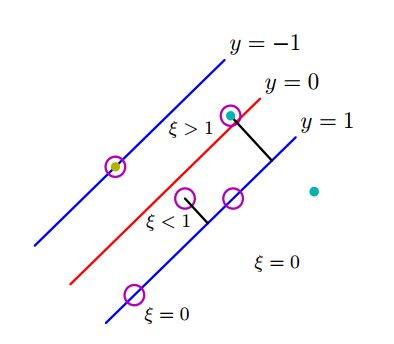
\includegraphics[scale=0.5]{img/1b.jpeg}
			\caption{توصیف معنایی حالات مختلف $\epsilon$}
		\end{figure}
		\item سه)
		حل مسئله با $M$ متغیر به طور کلی پیچیدگی از $O(M^3)$ دارد. در دوگان مسئله‌ی بهینه‌سازی را می‌خواهیم حل کنیم که به‌جای $M$ متغیر، $N$ متغیر دارد. برای تعداد ثابت توابع \lr{basis} چون که 
		$M < N$
		است، استفاده از روش دوگان  به دلیل سرعت کم‌تر خوب نیست. 
		
		استفاده روش دوگان به ما امکان استفاده از هسته‌ها را می‌دهد و می‌توانیم دسته‌بند حاشیه بیشینه 
		\footnote{\lr{maximum margin classifier}}
		را که ابعاد  ویژگی‌های آن بیش‌تر از تعداد نقاط است پیدا کنیم و بسیار کارا است و حتی جواب‌گوی مواقعی که تعداد ویژگی‌ها به بی‌نهایت میل می‌کند می‌باشد.
		\footnote{ر.ک صفجه ۳۲۹ کتاب}
		\item چهار)
		\begin{figure}[hbpt!]
			\centering
			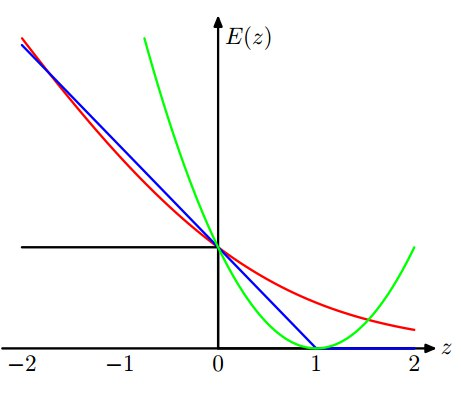
\includegraphics[scale=0.5]{./img/2.jpeg}
			\caption{نمودار آبی: ماشین بردار پشتیبان نرم، نمودار قرمز: 
			\lr{logistic regression}،
			نمودار مشکی: خطای دسته‌بندی
			و نمودار سبر: مربع خطاها
			}
		\end{figure}
		\begin{figure}[hbpt!]
			\centering
			\begin{tikzpicture}
				\begin{axis}[
				xlabel style={below right},
				xlabel=$x$,
				ylabel=$y$,
				ylabel style={above left},
				xmin=-2, xmax=2,
				ymin=0, ymax=2,
				axis lines=center,
				axis on top=true,
				domain=0:1,
				]
				
				\addplot+[color=red,mark=none,samples=200,domain=1:10,smooth,ultra thick] {0} node[below,pos=1,color=black] {};
				
				\addplot+[color=red,mark=none,samples=200,domain=-2:-0,smooth,ultra thick] {2} node[below,pos=1,color=black] {};
				\end{axis}
			\end{tikzpicture}
			\caption{ماشین بردار پشتیبان سخت}
		\end{figure}
	
		\begin{figure}[hbpt!]
			\centering
			\begin{tikzpicture}
			\begin{axis}[
			xlabel style={below right},
			xlabel=$x$,
			ylabel=$y$,
			ylabel style={above left},
			xmin=-2, xmax=2,
			ymin=0, ymax=2,
			axis lines=center,
			axis on top=true,
			domain=0:1,
			]
			
			\addplot+[color=blue,mark=none,samples=200,domain=-2:0,smooth,ultra thick] coordinates{(0, 1)  (-1, 2)}; 
			\addplot+[color=blue,mark=none,samples=200,domain=0:10,smooth,ultra thick] {0} node[below,pos=1,color=black] {};
			
			\end{axis}
			\end{tikzpicture}
			\caption{\lr{perceptron}}
		\end{figure}
	\end{itemize}
	\item ب) 
	در این رابطه حساسیت به داده‌های نویز بیش‌تر می‌شود؛‌ زیرا در مدل  هدف این است که وقتی مجموع مجذورات  را کمینه کنیم، بنابراین داده‌های کم‌تری باید به‌طور اشتباه دسته‌بندی شوند و داده‌های نویز اثر و وزن زیادی نسبت به حالت عادی تابع هزینه دارند. 
	\item پ)
	\begin{itemize}
		\item یک)
		$$
		\tilde{L}(a) = \Sigma_{n = 1}^N a_n - \frac{1}{2}\Sigma_{n=1}^N\Sigma_{m=1}^Na_na_mt_nt_mk(x_nm x_m)
		$$
		از آن‌جایی که تعداد داده‌ها ۵ است، بنابراین:
		\footnote{ر.ک. صفحه ۳۲۹ کتاب}
		$$
			\tilde{L}(a) = \Sigma_{n = 1}^5 a_n - \frac{1}{2}\Sigma_{n=1}^5\Sigma_{m=1}^5a_na_mt_nt_mk(x_nm x_m)
		$$
		$$
\tilde{L}(a) = \Sigma_{n = 1}^5 a_n - \frac{1}{2}(a_1^2-4a_1a_4 - 4a_1a_3 - 6a_1a_5 + a_2^2 - 2a_2a_3-4a_2a_4 + 5a_3^2 - 2a_2a_5 + 12a_3a_4 + 14a_3a_5 + 8a_4^2 + 16a_4a_5 + 10a_5^2)
		$$
		$$
		a_n \geq 0 \implies \Sigma_{n = 1}^N a_nt_n = 0 \implies a_1 + a_2 - a_3 - a_4 - a_5 = 0
		$$
		
		\item دو)
		\begin{figure}[hbpt!]
			\centering
			\begin{tikzpicture}
			\begin{axis}[
			axis lines=middle,
			xmin=-1, xmax=4,
			ymin=-1, ymax=4,
			xtick=\empty, ytick=\empty
			]
			\addplot [only marks] table {
				0 1
				1  0

			};
			\addplot [only marks, mark=o] table {
				1  2
				2  2
				1  3

			};
			\addplot [domain=-10:10, samples=2, dashed] {-1*x+2};
			\end{axis}
			\end{tikzpicture}
		\end{figure}
				چون نقطه‌‌های ۲، ۴ و ۵ نمی‌توانند بردار پشتیبان باشند، بنابراین داریم:
	$$
	a_2 = a_4 = a_5 = 0 \implies a_1 - a_3 = 0 \implies a_1 = a_3
	$$
		\item سه)
		با جای‌گذاری نتیجه‌ی بالا در معادله‌ی قسمت «۱» داریم:
		$$
		\tilde{L}(a) = 2a_1 - \frac{1}{2}(a_1^2 - 4a_1^2 + 5a_1^2) = -a_1^2 + 2a_1
		$$
		یا
			$$
		\tilde{L}(a) = 2a_3 - \frac{1}{2}(a_3^2 - 4a_3^2 + 5a_3^2) = -a_3^2 + 2a_3
		$$
		\item چهار)
		$$
		\tilde{L}(a)^{\prime} = -2a_3 + 2 = 0 \implies a_3 = 1
		$$
		\item پنج)
	\end{itemize}
\end{itemize}
